\documentclass{article}
\usepackage{amsmath}
\usepackage{fancyhdr}
\usepackage{amsmath}
\usepackage{clrscode}
\usepackage{subfigure}
\usepackage[top=3cm, bottom=3cm, left=3cm, right=3cm]{geometry}
\usepackage[pdftex]{graphicx}\title{BME511L: Lab3}
\usepackage{float}
\usepackage{amsfonts}
\author{Allen Yin}
\pagestyle{fancy}
\setlength\parindent{0.0in}
\setlength\parskip{0.0in}
\usepackage{caption}
\captionsetup{justification=justified}
\setcounter{tocdepth}{2}
\setlength{\headheight}{15pt}

\begin{document}
\maketitle
\setlength\parskip{0.1in}

\section{Question 4}

\begin{figure}[H]
    \begin{center}
        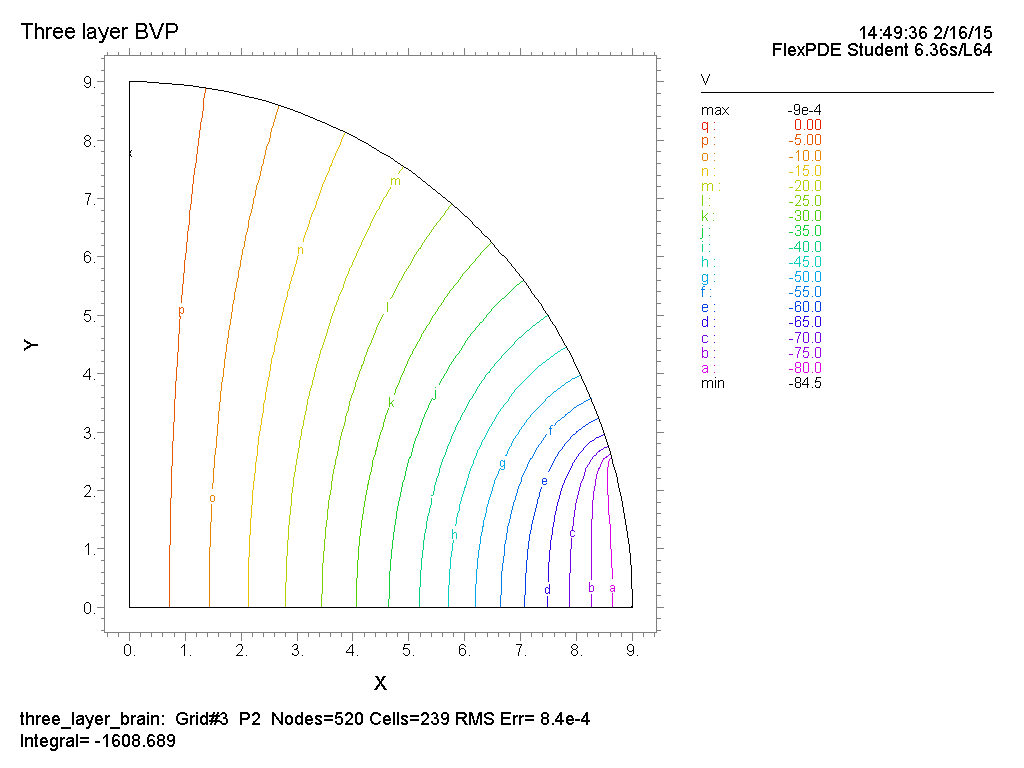
\includegraphics[scale=0.5]{homo_contourV.png}
        \caption{Contour plot of potential, homogeneous case}
    \end{center}
\end{figure}

\begin{figure}[H]
    \begin{center}
        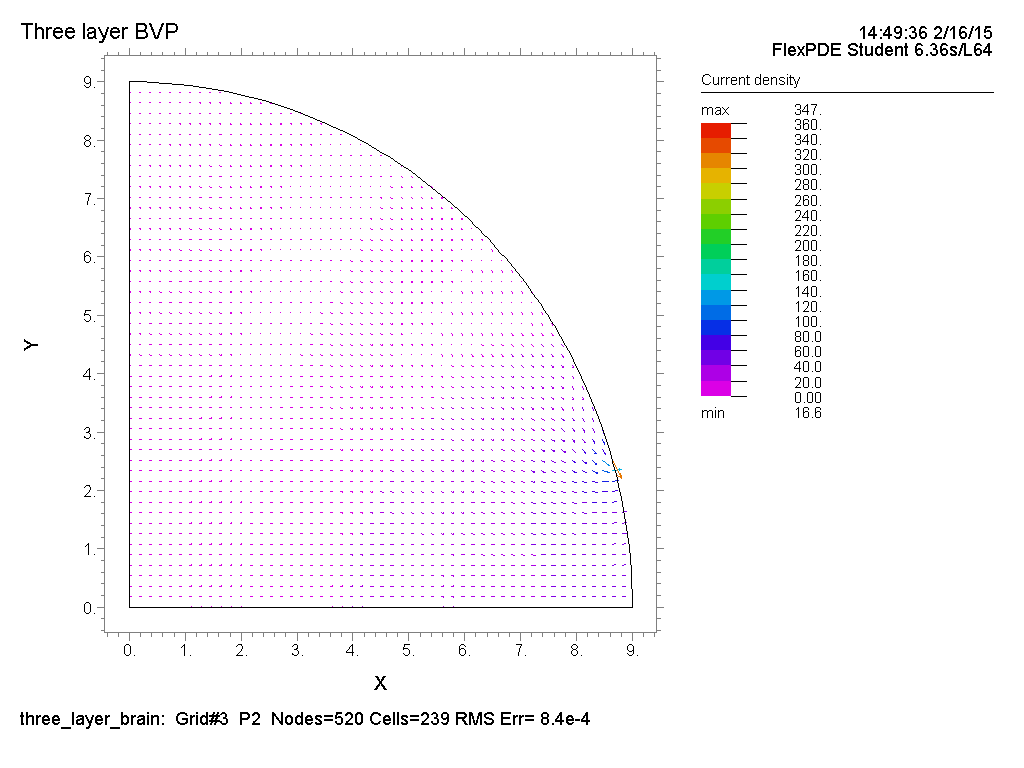
\includegraphics[scale=0.5]{homo_CD.png}
        \caption{Current density, homogeneous case}
    \end{center}
\end{figure}

\begin{figure}[H]
    \begin{center}
        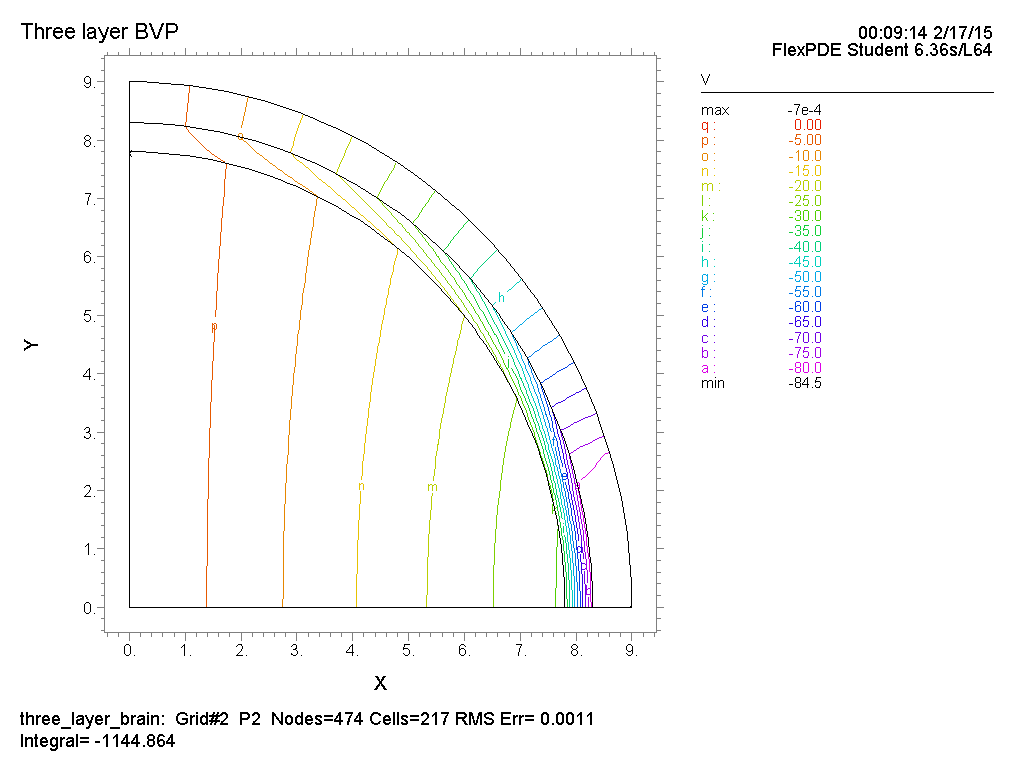
\includegraphics[scale=0.5]{contourV.png}
        \caption{Contour plot of potential, inhomogeneous case}
    \end{center}
\end{figure}

\begin{figure}[H]
    \begin{center}
        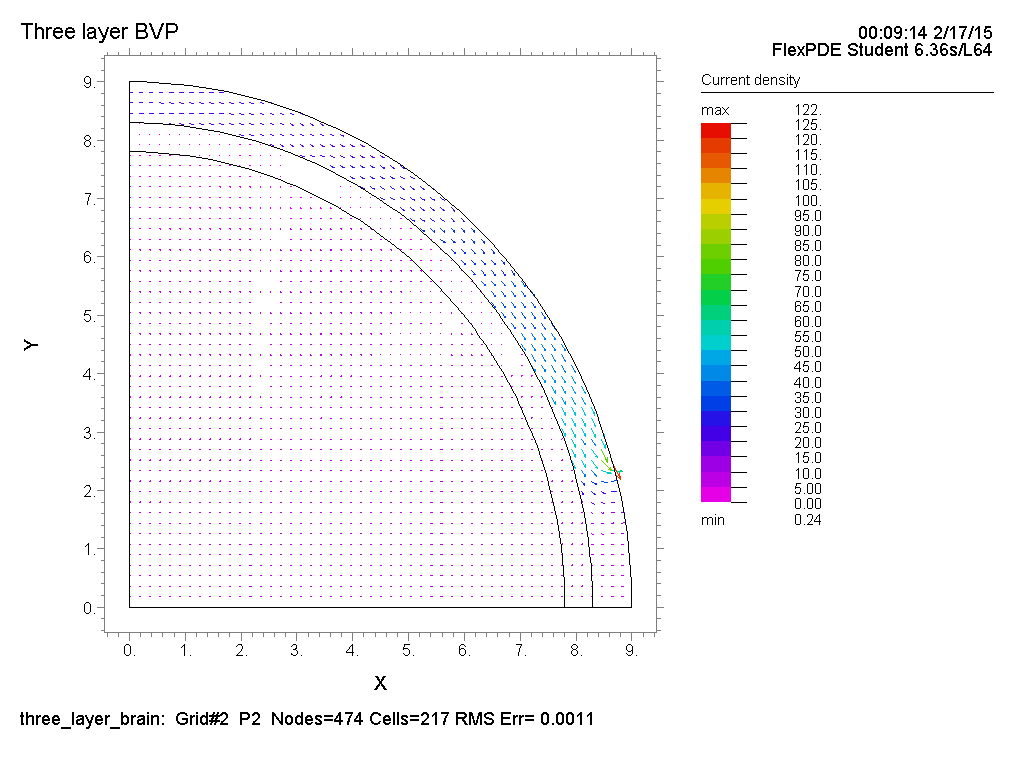
\includegraphics[scale=0.5]{CD.png}
        \caption{Current density, inhomogeneous case}
    \end{center}
\end{figure}

As seen in the figures, inhomogeneous conductivity distorts the equipotential lines and current density. Specifically, the low conductivity in the skull layer results in a sharp drop in potential level, and small current density.

\section{Question 5}
\begin{figure}[H]
    \begin{center}
    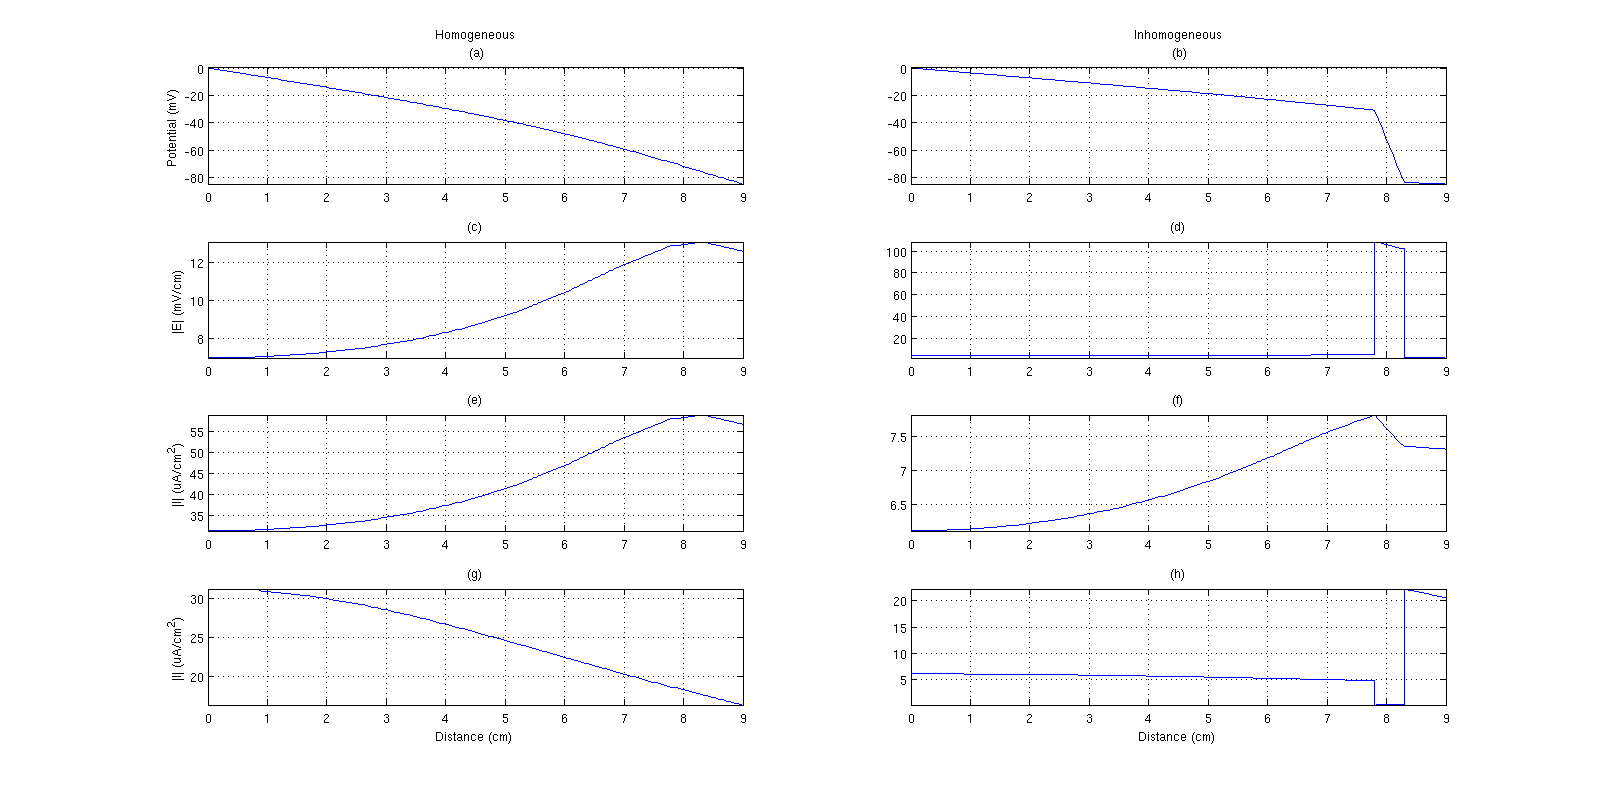
\includegraphics[scale=0.3]{comparison.png}
    \caption{Comparison of homogeneous vs. inhomogeneous quantities.\\  (a-b): Potential along the O-E. \\  (c-d): Tangential electric field along O-E. \\ (e-f): Tangentail current density along O-E. \\  (g-h): Normal current density along O-C.}
\end{center}
\end{figure}

\section{Question 6}
A line integral of the normal current density is done along the roughly 16 degrees arc where the electrode is located. 

For homogeneous case, this yields $204.6932\mu A/cm$, which leads to total current of $(204.6932\mu A/cm \times 2 \times 5cm=2046.932\mu A)$. 

For inhomogeneous case, this yields $46.4892\mu A/cm$, leading to $(46.4892\mu A/cm \times 2 \times 5cm = 464.892\mu A)$.

\section{Question 7}
The current tends to flow in the positive x-position toward the electrodes. This means the current density would be mainly tangential along O-E, and normal along O-C.

If we plotted normal curernt density along path O-E and tangential current density along path O-C, we would see 0 current density for most of the distances. This can be seen in the vector plot of current-density.

\section{Question 8}
In general, current density is greater in areas with greater conductivity. This can be seen through the current-density plots. As a result, the voltage drop within low conductivity regions also tend to be more rapid, this is visualized by the crowding of equipotential lines within the skull region in the inhomogeneous potential plot. Together, this results in less uniform current density vector direction in the different regions, visualized by the current density vector plot in the inhomogeneous case.

\end{document}
